\begin{tikzpicture}[
    font=\footnotesize,
    node/.style={draw, circle, fill=blue!20, inner sep=3pt, minimum size=30pt},
    traj/.style={inner sep=0pt},
    lstm/.style={draw, rectangle, fill=red!50, inner sep=2pt},
    localizer/.style={draw, rectangle, rounded corners, inner sep=0pt, fill=green!10},
    gnn/.style={draw, rectangle, rounded corners, fill=orange!20, inner sep=5pt},
    posterior/.style={draw, rectangle, rounded corners, inner sep=1pt},
    globalizer/.style={draw, rectangle, rounded corners, inner sep=0pt, fill=green!10},
    to/.style={->, ultra thick, -stealth},
    axis/.style={->,ultra thick, gray},
    axislabel/.style={text=black},
    anglearc1/.style={draw, thin, opacity=0.2, fill=red!50},
    anglearc2/.style={draw, thin, opacity=0.2, fill=cyan!50},
    anglearc3/.style={draw, thin, opacity=0.2, fill=orange!50},
    anglearc4/.style={draw, thin, opacity=0.2, fill=blue!50},
    separator/.style={thick, gray, dotted},
  ]

\begin{scope}[name prefix=t1-]
  % \node[node] (x_t_dec) {$\mathbf{x}^{t}$};
  \node[traj, label=above:Input Trajectories] (x_t_dec)
    {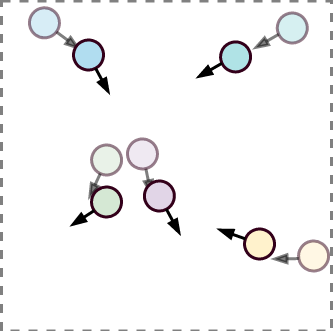
\includegraphics[width=.25\textwidth]{figures/pipeline/input_trajectories.png}};
  \node[localizer, right=of x_t_dec, label=above:Global\to Local] (g2l_dec)
    {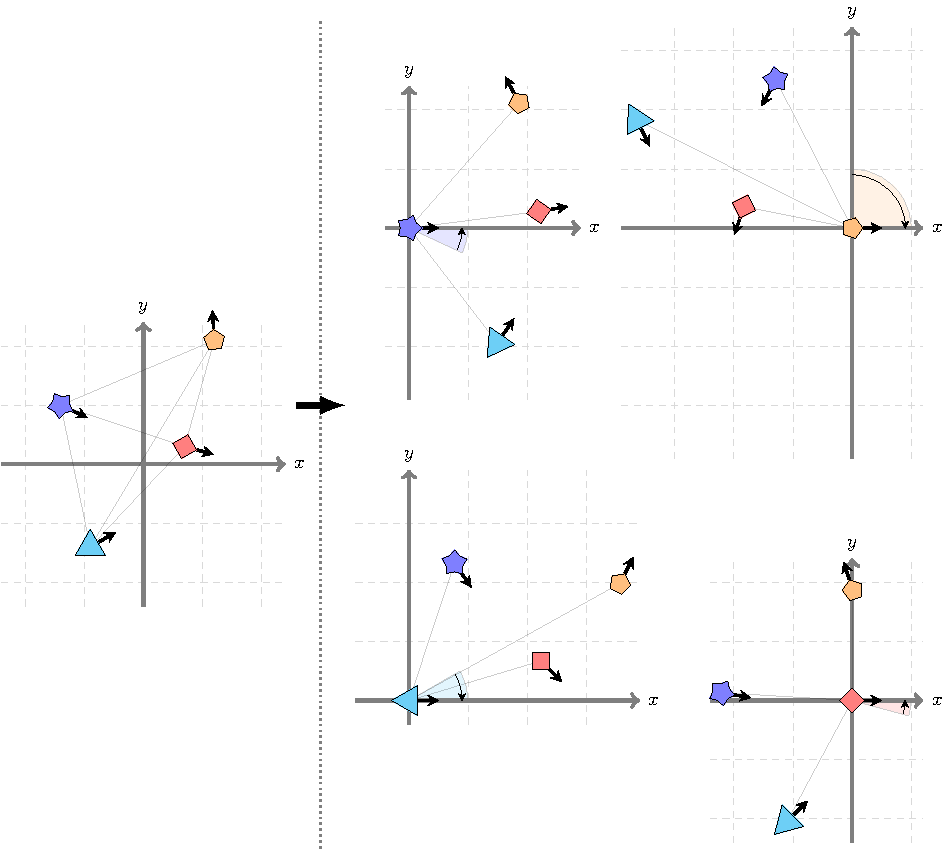
\includegraphics[width=.2\textwidth]{figures/locs/global_to_local.pdf}};
  \node[gnn, right=of g2l_dec, align=center] (gnn_dec) {Graph\\Neural Network};
  \node[globalizer, right=of gnn_dec, label=above:Local\to Global] (l2g_dec)
  {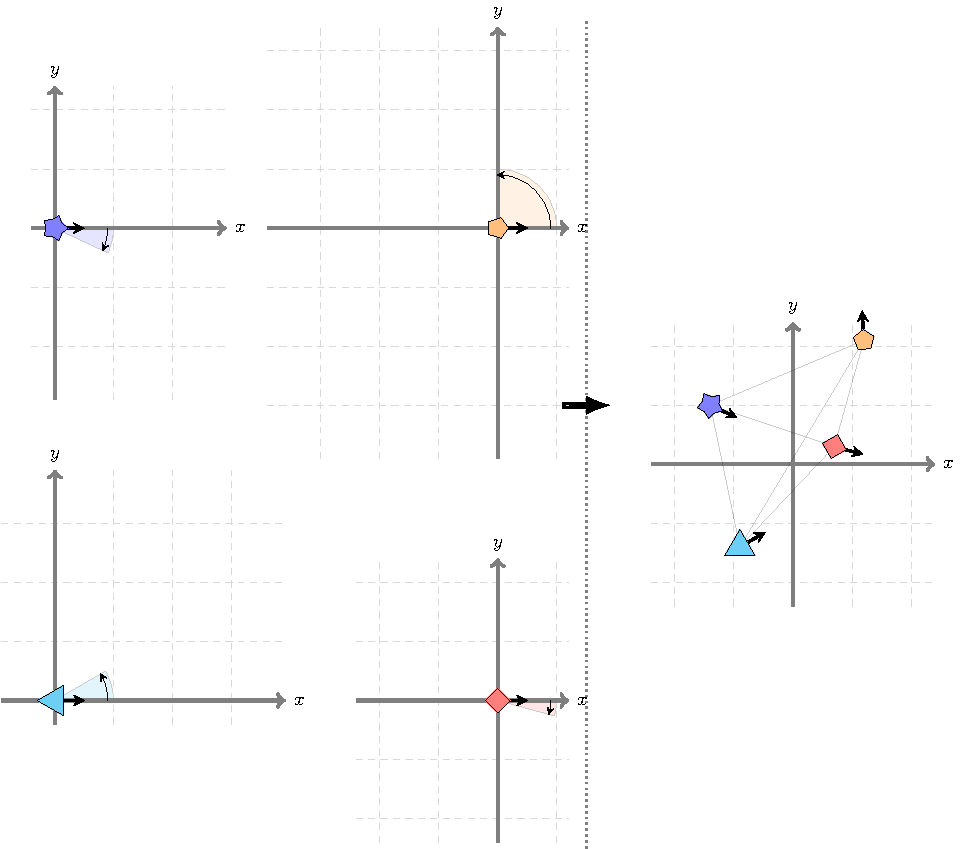
\includegraphics[width=.2\textwidth]{figures/locs/local_to_global.pdf}};
  \node[traj, right=of l2g_dec, label=above:Predicted Trajectories] (x_hat)
  {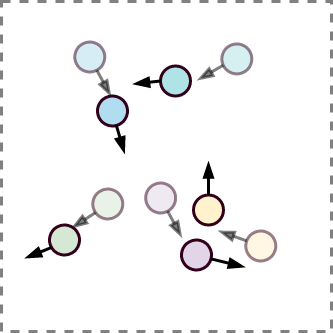
\includegraphics[width=.25\textwidth]{figures/pipeline/output_trajectories.png}};
  % \node[node, right=of l2g_dec] (x_hat) {$\mathbf{x}^{t+1}$};
  \node[fit=(g2l_dec)(gnn_dec)(l2g_dec), draw, rounded corners, opacity=0.3, inner ysep=24pt, label=below:LoCS \cite{kofinas2021roto}] (locs) {};

  \draw[to] (x_t_dec)--(g2l_dec);
  \draw[to] (g2l_dec)--(gnn_dec);
  \draw[to] (gnn_dec)--(l2g_dec);
  \draw[to] (l2g_dec)--(x_hat);
\end{scope}

\end{tikzpicture}
